\section{Teorema de Cauchy}
\subsection{El Teorema de Cauchy}

\begin{definición}[Triangulo en $\mathbb{C}$]
    Un triangulo en $\mathbb{C}$ es la envoltura convexa de tres puntos distintos no colineales de $\Omega$, $z_1, z_2, z_3 \in \Omega$:
    \[
        \Delta = \{ z \in \mathbb{C} : 
        z = t_1 z_1 + t_2 z_2 + t_3 z_3, \quad
        0 \leq t_i \leq 1, t_1 + t_2 + t_3 = 1 \}
    \]
    Denotaremos a la frontera del triángulo como $\partial \Delta$, y le llamaremos borde de $\Delta$. Además, asumimos orientación positiva en el borde (sentido antihorario).
\end{definición}

\begin{teorema}[Teorema de Cauchy para triángulos / Teorema de Cauchy-Goursat]
    Si $f: \Omega \subset \mathbb{C} \to \mathbb{C}$ es holomorfa en un abierto $\Omega$, entonces:
    \[
        \int_{\partial \Delta} f(z) \, dz = 0 \quad \forall \Delta \subset \Omega
    \]
\end{teorema}

\begin{proof}
    Sea $\Delta$ un triángulo en $\Omega$. Queremos probar que $I=\int_{\partial \Delta} f(z) \, dz = 0$, y para ello vamos a probar que $|I| \leq \varepsilon$ para todo $\varepsilon > 0$.\\
    En primer lugar dividimos $\Delta$ en $4$ triángulos usando los puntos medios de sus lados, y los llamaremos $\tilde{T}_1, \tilde{T}_2, \tilde{T}_3, \tilde{T}_4$. Entonces:

    \begin{center}
        \begin{tikzpicture}[scale=4]
            % Vertices
            \coordinate (A) at (0, 0);
            \coordinate (B) at (2, 0);
            \coordinate (C) at (2, 1);
    
            % Puntos medios
            \coordinate (M_AB) at ($(A)!0.5!(B)$);
            \coordinate (M_BC) at ($(B)!0.5!(C)$);
            \coordinate (M_CA) at ($(C)!0.5!(A)$);
    
            % Triángulo original
            \draw[thick] (A) -- (B) -- (C) -- cycle;
            \draw[thick, dashed] (M_AB) -- (M_BC) -- (M_CA) -- cycle;
            % Etiquetas
            \node at (A) [below left] {$z_1=A$};
            \node at (B) [below right] {$z_2=B$};
            \node at (C) [above right] {$z_3=C$};
            \node at (M_AB) [below] {$M_{12}=M_{AB}$};
            \node at (M_BC) [right] {$M_{23}=M_{BC}$};
            \node at (M_CA) [above left] {$M_{31}=M_{CA}$};
            % Flechas de orientación antihoraria en los bordes de los triángulos pequeños
            % Triángulo 1: (A, M_AB, M_CA) AZUL
            \draw[->, very thick, blue] ($(A)!0.5!(M_AB)$) -- ++(0.25,0);
            \draw[->, very thick, blue] ($(M_AB)!0.5!(M_CA)$) -- ++(0,0.15);
            \draw[->, very thick, blue] ($(M_CA)!0.5!(A)$) -- ++(-0.2,-0.1);
    
            % Triángulo 2: (M_AB, B, M_BC) ROJO
            \draw[->, very thick, red] ($(M_AB)!0.5!(B)$) -- ++(0.25,0);
            \draw[->, very thick, red] ($(B)!0.5!(M_BC)$) -- ++(0,0.2);
            \draw[->, very thick, red] ($(M_BC)!0.5!(M_AB)$) -- ++(-0.2,-0.1);
    
            % Triángulo 3: (M_CA, M_BC, C) VERDE
            \draw[->, very thick, green!60!black] ($(M_CA)!0.5!(M_BC)$) -- ++(0.15,0);
            \draw[->, very thick, green!60!black] ($(M_BC)!0.5!(C)$) -- ++(0,0.1);
            \draw[->, very thick, green!60!black] ($(C)!0.5!(M_CA)$) -- ++(-0.2,-0.1);
    
            % Triángulo central: (M_AB, M_BC, M_CA) NARANJA
            \draw[->, very thick, orange] ($(M_AB)!0.5!(M_BC)$) -- ++(0.2,0.1);
            \draw[->, very thick, orange] ($(M_BC)!0.5!(M_CA)$) -- ++(-0.15,0);
            \draw[->, very thick, orange] ($(M_CA)!0.5!(M_AB)$) -- ++(0,-0.15);
    
            % Nombres de los triángulos
            \node at ($(A)!0.33!(M_AB)!0.33!(M_CA)$) [blue] {$\tilde{T}_1$};
            \node at ($(M_AB)!0.33!(B)!0.33!(M_BC)$) [red] {$\tilde{T}_2$};
            \node at ($(M_CA)!0.33!(M_BC)!0.33!(C)$) [green!60!black] {$\tilde{T}_3$};
            \node at ($(M_AB)!0.33!(M_BC)!0.33!(M_CA)$) [orange] {$\tilde{T}_4$};
        \end{tikzpicture}
    \end{center}


    Teniendo en cuenta que $\int_{\gamma^-} f(z) \, dz = -\int_{\gamma} f(z) \, dz$, donde $\gamma^-$ es la curva $\gamma$ recorrida en sentido contrario, orientando todos los triángulos en sentido positivo es claro que:
    \[
        I = \int_{\partial \Delta} f(z) \, dz = \sum_{j=1}^{4} \int_{\partial \tilde{T}_j} f(z) \, dz
    \]
    Se cumple que al menos uno de los triángulos $\tilde{T}_j$, que llamaremos $T_1$, cumple que:
    \[
        \frac{|I|}{4} \leq \left| \int_{\partial T_1} f(z) \, dz \right|
    \]
    Así, 
    \[
        |I| \leq 4 \left| \int_{\partial T_1} f(z) \, dz \right| \quad \text{y} \quad \Long(\partial T_1) = \frac{\Long(\partial \Delta)}{2}
    \]
    Repitiendo lo anterior con $T_1$ en lugar de $\Delta$, obtenemos un triángulo $T_2 \subset T_1$ tal que:
    \[
        \left| \int_{\partial T_1} f(z) \, dz \right| \leq 4 \left| \int_{\partial T_2} f(z) \, dz \right| 
    \]
    y
    \[
        \Long(\partial T_2) = \frac{\Long(\partial T_1)}{2} = \frac{\Long(\partial \Delta)}{2^2}
    \]
    Reiterando el proceso obtenemos una sucesión de triángulos $(T_n)_{n \in \mathbb{N}}$ tal que:
    \begin{itemize}
        \item $T_{n+1} \subset T_n \quad \forall n \in \mathbb{N}$
        \item $|I| \leq 4^n \left| \int_{\partial T_n} f(z) \, dz \right| \quad \forall n \in \mathbb{N}$
        \item $\Long(\partial T_n) = \frac{\Long(\partial \Delta)}{2^n} \quad \forall n \in \mathbb{N}$
    \end{itemize}
    Como $(T_n)_{n \in \mathbb{N}}$ es una sucesión de conjuntos compactos encajados, tenemos que $\bigcap_{n=1}^{\infty} T_n \neq \emptyset$ (de hecho es un conjunto con un único punto).\\
    Sea $z_0 \in \bigcap_{n=1}^{\infty} T_n \subset \Omega$. Como $f$ es holomorfa en $\Omega$, es derivable en $z_0$, por tanto existe $\delta > 0$ tal que:
    \[
        \left| \frac{f(z) - f(z_0)}{z - z_0} - f'(z_0) \right| < \varepsilon \quad \forall z \in D(z_0, \delta) \setminus \{z_0\}
    \]
    luego $|f(z) - f(z_0) - f'(z_0)(z - z_0)| < \varepsilon |z - z_0|$ para todo $z \in D(z_0, \delta)\setminus \{z_0\}$.\\
    Teniendo en cuenta que $\lim_{n \to \infty} \Long(\partial T_n) = 0$, existe $N \in \mathbb{N}$ tal que $\Long(\partial T_n) < \delta$ para todo $n > N$. Ahora como $z_0 \in T_n$ para todo $n \in \mathbb{N}$, tenemos que $T_n \subset D(z_0, \delta)$ para todo $n > N$.\\
    Por tanto, 
    \[
        \left| f(z) - f(z_0) - f'(z_0)(z - z_0) \right| < \varepsilon |z - z_0| \quad \forall z \in \partial T_n, \ n > N
    \]
    Con lo cual, para todo $n > N$,
    \[
        \left| \int_{\partial T_n} f(z) \, dz \right|
        = \left| \int_{\partial T_n} \big( f(z) - f(z_0) - f'(z_0)(z - z_0) \big) dz 
        + \int_{\partial T_n} \big( f(z_0) + f'(z_0)(z - z_0) \big) dz \right|.
    \]
    Aplicando la desigualdad triangular,
    \[
        \leq \left| \int_{\partial T_n} \big( f(z) - f(z_0) - f'(z_0)(z - z_0) \big) dz \right|
        + \left| f(z_0) \int_{\partial T_n} 1 \, dz + f'(z_0) \int_{\partial T_n} (z - z_0) \, dz \right|.
    \]
    Observamos que ambas integrales del segundo término son nulas por el \cref{teo:existencia-primitivas}, ya que existen las primitivas de $1$ y de $z - z_0$ en $\mathbb{C}$:
    \[
        \int_{\partial T_n} 1 \, dz = [z]_{\partial T_n} = 0, 
        \qquad 
        \int_{\partial T_n} (z - z_0) \, dz = \left[ \tfrac{1}{2}(z - z_0)^2 \right]_{\partial T_n} = 0.
    \]
    Por tanto,
    \[
        \left| \int_{\partial T_n} f(z) \, dz \right|
        \leq \left| \int_{\partial T_n} \big( f(z) - f(z_0) - f'(z_0)(z - z_0) \big) dz \right|.
    \]
    Aplicando ahora la desigualdad M–L,
    \[
        \left| \int_{\partial T_n} \big( f(z) - f(z_0) - f'(z_0)(z - z_0) \big) dz \right|
        \leq \sup_{z \in \partial T_n} \left| f(z) - f(z_0) - f'(z_0)(z - z_0) \right|
        \cdot \Long(\partial T_n).
    \]
    Por la derivabilidad de $f$ en $z_0$, y manteniendo $n > N$, tenemos que
    \[
        \leq (\varepsilon \, \Long(\partial T_n)) \cdot \Long(\partial T_n)
        = \varepsilon \, (\Long(\partial T_n))^2.
    \]
    
    Finalmente
    \[
        |I| \leq 4^n \left| \int_{\partial T_n} f(z) \, dz \right| \leq 4^n \varepsilon (\Long(\partial T_n))^2 = 4^n \varepsilon \left( \frac{\Long(\partial \Delta)}{2^n} \right)^2 = \varepsilon (\Long(\partial \Delta))^2 
    \]
    Como $\varepsilon > 0$ es arbitrario, hemos probado que
    \[
        |I| \leq \varepsilon \Long(\partial \Delta)^2 \quad \forall \varepsilon > 0 \implies I = 0
    \]
\end{proof}

\textbf{Nota: } Usamos en la demostración que si $(K_n)_{n \in \mathbb{N}}$ es una sucesión de compactos no vacios y encajados entonces $\bigcap_{n=1}^{\infty} K_n \neq \emptyset$. Veamos la demostración de este hecho:

\begin{proof}
    Si:
    \[
    \bigcap_{n=1}^{\infty} K_n = \emptyset \implies
    \left( \bigcap_{n=1}^{\infty} K_n \right)^c =
    \bigcup_{n=1}^{\infty} K_n^c = \mathbb{C}
    \]
    Como $\{ K_n^c : n \in \mathbb{N} \}$ es una familia de abiertos que cubren a $\mathbb{C}$, y por tanto a $K_1$, como este es compacto existen $n_1 < n_2 < \ldots < n_m$ tales que $K_1 \subset \bigcup_{i=1}^{m} K_{n_i}^c$.\\
    Por un lado:
    \[
    \emptyset \neq K_{n_m} \subset K_1 \subset \bigcup_{i=1}^{m} K_{n_i}^c
    \]
    Luego si $x \in K_{n_m}$ existe $j_0 \in \{1, \ldots, m\}$ tal que $x \in K_{n_{j_0}}^c$, es decir, $x \notin K_{n_{j_0}}$.\\
    Por otro lado, como $K_{n_m} \subset K_{n_{j_0}}$ (pues la sucesión es encajada y $n_{j_0} \leq n_m$), tenemos que $x \in K_{n_{j_0}}$, lo cual es una contradicción.\\
    Por tanto, $\bigcap_{n=1}^{\infty} K_n \neq \emptyset$.
\end{proof}

\begin{teorema}[Teorema de Cauchy para convexos]
    Sea $f: \Omega \subset \mathbb{C} \to \mathbb{C}$ holomorfa en un abierto y convexo $\Omega$. Entonces, para cualquier curva cerrada $\gamma$ en $\Omega$:
    \[
        \int_{\gamma} f(z) \, dz = 0
    \]
\end{teorema}

\begin{proof}
    Si fijamos $z_0 \in \Omega$, como $\Omega$ es convexo, para cualquier $z \in \Omega$ el segmento que une $z_0$ y $z$ está contenido en $\Omega$. Por tanto, podemos definir:
    \[
    F : \Omega \to \mathbb{C}
    \]
    \[
        F(z) = \int_{[z_0, z]} f(w) \, dw
    \]
    Veamos que $F$ es derivable en $\Omega$ y que $F'(z) = f(z)$.\\
    Para ello fijemos $z_1 \in \Omega$ arbitrario, y como $\Omega$ es abierto existe $r > 0$ tal que $D(z_1, r) \subset \Omega$. Para cada $h \in \mathbb{C} : |h| < r$ tenemos que:
    \[
        \left| \frac{F(z_1 + h) - F(z_1)}{h} - f(z_1) \right| =
        \frac{1}{|h|} 
        \left|
        \int_{[z_0, z_1 + h]} f(w) \, dw - 
        \int_{[z_0, z_1]} f(w) \, dw -
        (h(f(z_1)))
        \right|
        =^*
    \]
    Aplicando el teorema, ya que $\int_{[z_0, z_1]} f(w) \, dw + \int_{[z_1, z_1 + h]} f(w) \, dw - \int_{[z_0, z_1 + h]} f(w) \, dw = 0$:
    \begin{center}
        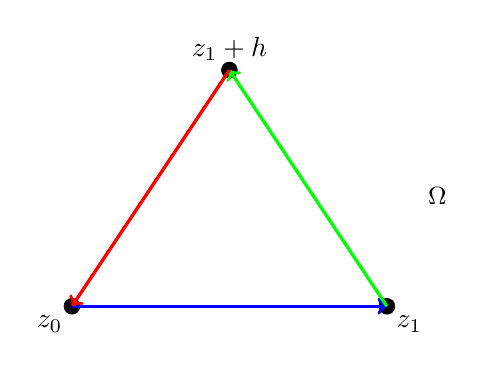
\begin{tikzpicture}[scale=2]
            % Vertices
            \coordinate (A) at (0,0);
            \coordinate (B) at (2,0);
            \coordinate (C) at (1,1.5);

            % Draw triangle
            \draw[thick] (A) -- (B) -- (C) -- cycle;

            % Points
            \fill (A) circle (1.5pt);
            \fill (B) circle (1.5pt);
            \fill (C) circle (1.5pt);

            % Labels
            \node[below left] at (A) {$z_0$};
            \node[below right] at (B) {$z_1$};
            \node[above] at (C) {$z_1 + h$};

            % Path [z_0, z_1], [z_1, z_1+h], [z_1+h, z_0]
            \draw[->, very thick, blue] (A) -- (B);
            \draw[->, very thick, green] (B) -- (C);
            \draw[->, very thick, red] (C) -- (A);

            % Legend
            \node[right] at (2.2,0.7) {\small $\Omega$};
        \end{tikzpicture}
    \end{center}

    El triángulo con vértices $z_0$, $z_1$ y $z_1 + h$ está contenido en $\Omega$ por convexidad, por lo que podemos aplicar el Teorema de Cauchy-Goursat a la integral sobre su borde:
    \[
    \int_{[z_0, z_1]} f(w)\,dw + \int_{[z_1, z_1+h]} f(w)\,dw + \int_{[z_1+h, z_0]} f(w)\,dw = 0
    \]
    \[
        =^*
        \frac{1}{|h|} 
        \left|
        \int_{[z_1, z_1 + h]} f(w) \, dw -
        \int_{[z_1, z_1 + h]} f(z_1) \, dw
        \right| =
        \frac{1}{|h|}
        \left|
        \int_{[z_1, z_1 + h]} (f(w) - f(z_1)) \, dw
        \right| \leq
    \]
    \[
    \leq
    \frac{1}{|h|}
    \left(
        \max_{w \in [z_1, z_1 + h]} |f(w) - f(z_1)| 
    \right) \cdot
    \underbrace{\left(\Long ([z_1, z_1 + h])\right)}_{=|h|}
     =
    \max_{w \in [z_1, z_1 + h]} |f(w) - f(z_1)| \to 0 \quad \text{cuando } h \to 0
    \]
    Esto tiende a $0$ cuando $h \to 0$ por la continuidad de $f$ en $z_1$.\\
    Por tanto, $F$ es derivable en $z_1$ y $F'(z_1) = f(z_1)$. Como $z_1$ era arbitrario, $F$ es holomorfa en $\Omega$ y $F' = f$.\\
\end{proof}

Así, por este teorema, toda función holomorfa en un abierto convexo tiene primitiva en dicho abierto. En particular, toda función holomorfa en un abierto convexo $\Omega$ tiene primitiva en cada subconjunto abierto y convexo de $\Omega$.\\

El resultado anterior tiene aplicaciones interesantes aunque $\Omega$ no sea convexo:

\ejemplo{
    \begin{enumerate}
        \item Sea $f \in \mathcal{H}(\mathbb{C} \setminus \{0\})$, y $C_1, C_2$ dos circunferencias centradas en el origen y orientadas positivamente, entonces:
        \[
            \int_{C_1} f(z) \, dz = \int_{C_2} f(z) \, dz
        \]
        \begin{center}
            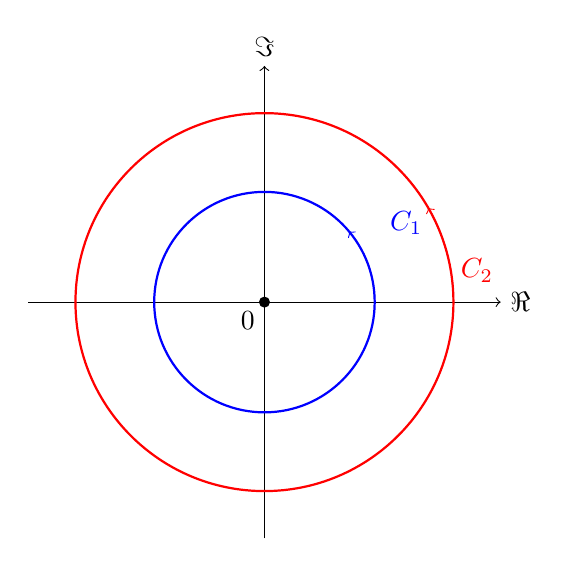
\begin{tikzpicture}[scale=2]
                % Ejes
                \draw[->] (-1.5,0) -- (1.5,0) node[right] {$\Re$};
                \draw[->] (0,-1.5) -- (0,1.5) node[above] {$\Im$};
                % Circunferencia C1
                \draw[thick, blue] (0,0) circle (0.7);
                \node[blue] at (0.9,0.5) {$C_1$};
                % Circunferencia C2
                \draw[thick, red] (0,0) circle (1.2);
                \node[red] at (1.35,0.2) {$C_2$};
                % Origen
                \fill (0,0) circle (1pt);
                \node[below left] at (0,0) {$0$};
                % Flechas de orientación positiva
                \draw[->, blue] (0.7,0) arc (0:40:0.7);
                \draw[->, red] (1.2,0) arc (0:30:1.2);
            \end{tikzpicture}
        \end{center}
        Podemos definir los caminos de cada circunferencia en cada sector, por ejemplo $\Gamma_1 \subset \{ z = x + iy : x > 0, y > 0 \}$, que además unen $C_1$ y $C_2$. Y como cada sector es convexo, podemos aplicar el teorema de Cauchy para convexos en cada sector, y sumar las integrales:
        \[
            0 =
            \sum_{i=1}^{4} \int_{\Gamma_i} f(z) \, dz =
            \int_{C_2} f(z) \, dz + \int_{C_1^-} f(z) \, dz =
            \int_{C_2} f(z) \, dz - \int_{C_1} f(z) \, dz
        \]
        Por tanto podemos obtener que las integrales son iguales: $\int_{C_1} f(z) \, dz = \int_{C_2} f(z) \, dz$.\\
        Esto además nos ayuda a calcular la integral de cualquier curva al rededor del origen, ya que es igual a la integral sobre cualquier circunferencia centrada en el origen, la cual sera mas facil de calcular.
        \begin{center}
            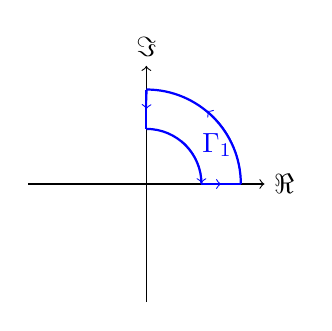
\begin{tikzpicture}
                % Ejes
                \draw[->] (-1.5,0) -- (1.5,0) node[right] {$\Re$};
                \draw[->] (0,-1.5) -- (0,1.5) node[above] {$\Im$};

                \draw[thick, blue] (0.7,0) arc (0:90:0.7);
                \draw[thick, blue] (0,0.7) -- (0,1.2);
                \draw[thick, blue] (1.2,0) -- (0.7,0);
                \draw[thick, blue] (1.2,0) arc (0:90:1.2);
                \draw[<-, blue] (0.7,0.01) arc (0:50:0.7);
                \draw[->, blue] (0.01,1.2) -- (0,0.95);
                \draw[->, blue] (1.2,0.01) arc (0:50:1.2);
                \draw[->, blue] (0.71,0) -- (0.95,0);
                \node[blue] at (0.9,0.5) {$\Gamma_1$};
            \end{tikzpicture}
        \end{center}
        \item Sea $f \in \mathcal{H}(\mathbb{C} \{0\})$ y $\gamma$ una curva cerrada en $\mathbb{C} \setminus \{0\}$, entonces:
        \[
            \int_{\gamma} f(z) \, dz = 0
        \]
        \item El abierto $\Omega = \mathbb{C} \setminus (-\infty, 0]$ no es convexo, pero aunasi para toda curva cerrada $\gamma$ en $\Omega$ y $f \in \mathcal{H}(\Omega)$ se cumple que:
        \[
            \int_{\gamma} f(z) \, dz = 0
        \]
    \end{enumerate}
}

\textbf{Nota:} El teorema anterior es equivalente a que si $\Omega \subset \mathbb{C}$ es abierto y convexo y $f: \Omega \to \mathbb{C}$ es holomorfa en $\Omega$, entonces
\[
    \int_{\gamma_1} f(z) \, dz = \int_{\gamma_2} f(z) \, dz \quad \forall \gamma_1, \gamma_2 \subset \Omega \text{ caminos con los mismo extremos}
\]

En vista del toerema de Cauchy para convexos vamos a poder definir $\int_{\gamma} f(z) \, dz$ para cualquier función $f$ continua en $\gamma^*$ siendo $\gamma : [a, b] \to \mathbb{C}$ una curva en $\mathbb{C}$ continua, sin necesidad de que $\gamma$ sea $\mathcal{C}^1$ ó $\mathcal{C}^1$ a trozos.

\begin{lema}
    Sea $\Omega \subset \mathbb{C}$ un abierto y $K \subset \Omega$ compacto, entonces existe $r > 0$ tal que:
    \[
        \Omega_0 = \bigcup_{z \in K} D(z, r) \ \text{ es subconjunto abierto de } \Omega
    \]
    que, además, es conexo si $K$ lo es, y es convexo si $K$ lo es.
\end{lema}

\begin{proof}
    \leavevmode
    \begin{itemize}
        \item Si $\Omega = \mathbb{C}$ cualquier $r > 0$ lo cumple pues es claro que $\Omega_0 \subset \mathbb{C}$ y que $\Omega_0$ es abierto (por ser unión de abiertos).\\
        Si $K$ es conexo entonces
        \[
            \Omega_0 = K \cup \left(\bigcup_{z \in K} D(z, r)\right) 
        \]
        Como $K \cap D(z, r) \neq \emptyset$ para todo $z \in K$, y tanto $K$ como $D(z, r)$ son conexos, deducimos, por el teorema del pivote que $\Omega_0$ es conexo.\\
        Y si $K$ es convexo, entonces $\Omega_0$ lo es también pues $\Omega_0 = K + D(0, r)$, y la suma de conjuntos convexos es convexa.\\
        \item Si $\Omega \subsetneq \mathbb{C}$ entonces $\Omega^c = \mathbb{C} \setminus \Omega \neq \emptyset$. Definimos
        \[
            \begin{matrix}
                \varphi : K \to \mathbb{R} \\
                z \mapsto \min_{w \in \Omega^c} |z - w|
            \end{matrix}
        \]
        ese mínimo existe, pues nos podemos restringir a un disco de radio suficientemente grande.\\
        $\varphi : K \to \mathbb{R}$ es continua, y $K$ es compacto, luego $\exists z_0 \in K$ tal que $\varphi(z_0) \leq \varphi(z) \ \forall z \in K$.\\
        Como $z_0 \in K \subset \Omega$, y $\Omega$ es abierto, existe $\delta > 0$ tal que $D(z_0, \delta) \subset \Omega$. Por tanto, $\varphi(z_0) \geq \delta > 0$.\\
        Sea $r = \frac{\varphi(z_0)}{2} > 0$, entonces tenemos que 
        \[
            \Omega_0 = \bigcup_{z \in K} D(z, r) \subset \Omega
        \]
    \end{itemize}    
\end{proof}

\begin{lema}
    Sea $\Omega \subset \mathbb{C}$ un abierto y sea $\gamma : [a, b] \to \Omega$ una curva continua en $\Omega$ (no necesariamente $\mathcal{C}^1$ ni $\mathcal{C}^1$ a trozos), entonces existe $\{t_0, t_1, \ldots, t_n\}$ partición de $[a, b]$ tal que para cada $j \in \{1, \ldots, n\}$, $\gamma([t_{j-1}, t_j])$ está contenida en un disco $D_j \subset \Omega$.
\end{lema}

\begin{proof}
    Como $\gamma : [a, b] \to \Omega$ es continua, entonces $\gamma^* = \gamma([a, b]) \subset \Omega$ es compacto y conexo. Por el lema anterior existe $r > 0$ tal que:
    \[
        \gamma^* \subset \Omega_0 = \bigcup_{t \in [a,b]} D(\gamma(t), r) \subset \Omega
    \]
    $\gamma$ continua en $[a, b]$ compacto, luego $\gamma$ es uniformemente continua en $[a, b]$. Por tanto, para $\frac{r}{2} > 0$ existe $\delta > 0$ tal que si $|t - t'| < \delta$ entonces $|\gamma(t) - \gamma(t')| < \frac{r}{2}$.\\
    Tomamos $\{t_0, t_1, \ldots, t_n\}$ partición de $[a, b]$ tal que $|t_j - t_{j-1}| < \delta$ para todo $j \in \{1, \ldots, n\}$.\\
    Así, 
    \[
        \gamma ([t_{j-1}, t_j]) \subset \underbrace{D \left(\gamma(t_{j}), \frac{r}{2}\right) }_{D_j} \subset \Omega \quad \forall j \in \{1, \ldots, n\}
    \]
\end{proof}

Veamos cómo definir $\int_{\gamma} f(z) \, dz$ donde $\gamma : [a,b] \to \Omega$ es una curva continua en $\Omega$ y $f \in \mathcal{H}(\Omega)$. Por el lema anterior existe una partición $\{t_0, t_1, \ldots, t_n\}$ de $[a, b]$ tal que para cada $j \in \{1, \ldots, n\}$, $\exists D_j \subset \Omega$ disco tal que $\gamma([t_{j-1}, t_j]) \subset D_j$.
\[
    f(z) \in \mathcal{H}(\Omega) \implies f(z) \in \mathcal{H}(D_j) \text{ para } j = 1, \ldots, n
\]  
Luego por el teorema de Cauchy para convexos, $\exists F_j : D_j \to \mathbb{C}$ primitiva de $f$ en $D_j$. Así podemos definir:
\[
    \int_{\gamma} f(z) \, dz = \sum_{j=1}^{n} \int_{\gamma|_{[t_{j-1}, t_j]}} f(z) \, dz = \sum_{j=1}^{n} (F_j(\gamma(t_j)) - F_j(\gamma(t_{j-1})))
\]

\begin{definición} [Deformación elemental]
Sea $\gamma : [a, b] \to \mathbb{C}$ una curva en $\Omega \subset \mathbb{C}$. Si $\tilde{\gamma} : [a,b] \to \Omega$ es otra curva tal que $\exists t_1, t_2 \in [a,b]$ con $t_1 < t_2$ tal que $\tilde{\gamma}(t) \equiv \gamma$ en $[a, t_1) \cup (t_2, b]$ y $\exists \Omega_0$ subconjunto abierto convexo de $\Omega$ tal que 
\[
    \gamma([t_1, t_2]) \cup \tilde{\gamma}([t_1, t_2]) \subset \Omega_0
\]
entonces decimos que $\tilde{\gamma}$ es una \textbf{deformación elemental} de $\gamma$ en $\Omega$.
\end{definición}

\begin{proposición}
    Sea $\Omega \subset \mathbb{C}$ un abierto y $f \in \mathcal{H}(\Omega)$. Si $\gamma_1, \gamma_2$ son curvas en $\Omega$ tales que $\gamma_2$ se obtiene con un número finito de deformaciones elementales de $\gamma_1$, entonces
    \[
        \int_{\gamma_1} f(z) \, dz = \int_{\gamma_2} f(z) \, dz
    \]
\end{proposición}

\begin{proof}
    Se prueba por inducción sobre el número de deformaciones elementales de $\gamma_1$, teniendo en cuenta que $\gamma_2$ es una deformación elemental de $\gamma_1$. Entonces
    \[
        \int_{\gamma_1} f(z) \, dz = \int_{\gamma_1|_{[a, t_1]}} f(z) \, dz + \int_{\gamma_1|_{[t_1, t_2]}} f(z) \, dz + \int_{\gamma_1|_{[t_2, b]}} f(z) \, dz 
    \]
    Como $\gamma_1 |_{[t_1, t_2]}$ y $\gamma_2 |_{[t_1, t_2]}$ son curvas con los mismos extremos, contenidas en $\Omega_0$ abierto y convexo ($f$ holomorfa en $\Omega$), tenemos:
    \[
        \int_{\gamma_1|_{[t_1, t_2]}} f(z) \, dz = \int_{\gamma_2|_{[t_1, t_2]}} f(z) \, dz = F(\gamma_1(t_2)) - F(\gamma_1(t_1))
    \]
    siendo $F : \Omega_0 \to \mathbb{C}$ una primitiva de $f$ en $\Omega_0$. 
\end{proof}

\subsection{Curvas homótopas}

\begin{definición}[Curvas homótopas]
    Sea $\Omega \subset \mathbb{C}$ un abierto y sean $\gamma, \tilde{\gamma}$ dos curvas en $\Omega$ con extremos $a,b$. Diremos que $\gamma$ y $\tilde{\gamma}$ son \textbf{homótopas} en $\Omega$ si:
    \[
    \exists \phi : [0,1] \times [0,1] \to \Omega
    \]   
    Una función continua que cumple:
    \[
    \begin{array}{rl}
        \phi(0, s) = a & \forall s \in [0,1] \\
        \phi(1, s) = b & \forall s \in [0,1] \\
        \phi(t, 0) = \gamma(t) & \forall t \in [0,1] \\
        \phi(t, 1) = \tilde{\gamma}(t) & \forall t \in [0,1] \\ 
    \end{array}
    \]
    Y lo denotaremos por:
    \[
    \gamma \sim \tilde{\gamma}
    \]
\end{definición}

\begin{definición}[Curva homótopa a $0$]
    Diremos que una curva cerrada $\gamma : [0,1] \to \Omega$ es \textbf{homótopa a $0$} en $\Omega$ si $\gamma$ es homótopa en $\Omega$ a la curva constante $\gamma_0(t) \equiv \gamma(0)$.
\end{definición}

\ejemplo{
    $C(2i, 1) \sim 0$ en $\Omega = \mathbb{C} \setminus \{0\}$, pero $C(0,1) \not\sim 0$ en $\Omega = \mathbb{C} \setminus \{0\}$ (pero si en $\Omega = \mathbb{C}$)
}

\begin{lema}[Lema 3]
    Sea $\Omega \subset \mathbb{C}$ un abierto y sean $\gamma \sim \tilde{\gamma}$ dos curvas homótopas en $\Omega$. Entonces $\tilde{\gamma}$ se obtiene de $\gamma$ mediante un número finito de deformaciones elementales en $\Omega$.
\end{lema}

\begin{proof}
    Sea $\phi : [0,1] \times [0,1] \to \Omega$ la función continua que define la homotopía entre $\gamma$ y $\tilde{\gamma}$.\\
    Como $[0,1] \times [0,1]$ es compacto y $\phi$ es continua (es más, uniformemente continua al serlo en un compacto), $\phi([0,1]^2) \subset \Omega$ es compacto. Por tanto, por el lema $1$, $\exists r > 0$ tal que:
    \[
        \phi([0,1]^2) \subset
        \Omega_0 =
        \bigcup_{(t,s) \in [0,1]^2} D(\phi(t,s), r) \subset 
        \Omega
    \]
    Como $\phi$ es uniformemente continua, $\exists \delta > 0$ tal que si:
    \[
    (t,s),(t',s') \in [0,1]^2, \quad
    \lVert (t,s) - (t',s') \rVert_2 < \delta \implies
    |\phi(t,s) - \phi(t',s')| < r
    \]
    Tomemos $n \in \mathbb{N}$ tal que $\frac{\sqrt{2}}{n} < \delta$, y dividamos $[0,1] \times [0,1]$ en $n^2$ cuadrados de lado $\frac{1}{n}$, y llamémosles $R_k: 1 \leq k \leq n^2$.\\
    Esta claro que $2$ puntos de $R_k$ cualesquiera están a distancia menor que $\frac{\sqrt{2}}{n}$, luego sus imágenes por $\phi$ distan menos de $r$.\\
    Eligiendo por ejemplo $z_k = (t_k,s_k) \in R_k$ el vértice inferior izquierdo de $R_k$, tenemos que:
    \[
        \phi(R_k) \subset D(\phi(z_k), r) \subset \Omega
    \]
    Finalmente, para cada $m \in \{1, \ldots, n\}$, 
    \[
        \begin{matrix}
            \gamma_m : [0,1] \to \Omega \\
            t \mapsto \phi(t, \frac{m}{n})
        \end{matrix}
    \]
    se obtiene a partir de $\gamma_{m-1}$ mediante $n$ deformaciones elementales en $\Omega$.
\end{proof}

\begin{teorema} [Teorema de Cauchy para curvas homótopas]
    Sea $\Omega \subset \mathbb{C}$ un abierto y $f \in \mathcal{H}(\Omega)$. Entonces 
    \[
        \int_{\gamma} f(z) \, dz = 0
    \]
    para toda curva cerrada $\gamma$ en $\Omega$ homótopa a $0$ en $\Omega$.
\end{teorema}

\begin{proof}
    $\gamma \sim 0$ en $\Omega \iff \gamma \sim \gamma_0 \equiv \gamma(0)$ en $\Omega \implies$ por el lema 3, $\gamma_0$ se obtiene de $\gamma$ mediante un número finito de deformaciones elementales en $\Omega$.\\
    Por la proposición anterior, 
    \[
        \int_{\gamma} f(z) \, dz = \int_{\gamma_0} f(z) \, dz = \int_{t=0}^{t=1} f(\gamma(0)) \cdot 0 \, dt = 0
    \]
    donde 
    \[
        \begin{matrix}
            \gamma_0 : [0,1] \to \Omega \\
            t \mapsto \gamma(0)\\
        \end{matrix} \quad \gamma'_0(t) = 0 \quad \forall t \in [0,1]
    \]
\end{proof}

\textbf{Nota:} El teorema anterior nos dice que si $\gamma_1, \gamma_2$ son curvas en $\Omega$ y $f \in \mathcal{H}(\Omega)$, entonces:
\[
    \int_{\gamma_1} f(z) \, dz = \int_{\gamma_2} f(z) \, dz \quad \text{puesto que }\gamma_1 \cup \gamma_2^- \sim 0 \text{ en } \Omega
\]

\begin{proposición}[Propiedades elementales]
    Sea $\Omega \subset \mathbb{C}$ un abierto:
    \begin{enumerate}
        \item "Ser homótopas en $\Omega$" es una relación de equivalencia entre curvas en $\Omega$ con los mismos extremos.
        \item Si $\varphi : [0,1] \to [0,1]$ continua con $\varphi(0) = 0$ y $\varphi(1) = 1$, entonces para toda curva $\gamma$ en $\Omega$ se cumple que $\gamma \sim \gamma \circ \varphi$ en $\Omega$. Esto se puede probar considerando:
        \[
        \phi (t,s) = \gamma((1 - s)t + s \varphi(t))
        \]
        \item Si $\gamma_1 \sim \tilde{\gamma}_1$ en $\Omega$ y $\gamma_2 \sim \tilde{\gamma}_2$ en $\Omega$, tal que el extremo final de $\gamma_1$ es el extremo inicial de $\gamma_2$, entonces:
        \[
            \left( \gamma_1 \cup \gamma_2 \right) \sim \left( \tilde{\gamma}_1 \cup \tilde{\gamma}_2 \right) \text{ en } \Omega
        \]
        \item Si $g: \Omega \to \widetilde{\Omega}$ es un homeomorfismo entre $2$ abiertos $\Omega, \widetilde{\Omega} \subset \mathbb{C}$, y si $\gamma, \tilde{\gamma}$ son curvas en $\Omega$ homótopas en $\Omega$, entonces:
        \[
            \left( g \circ \gamma \right) \sim \left( g \circ \tilde{\gamma} \right) \text{ en } \widetilde{\Omega}
        \]
        Esto se prueba ya que $\gamma \sim \tilde{\gamma}$ en $\Omega \implies \exists \phi : [0,1] \times [0,1] \to \Omega$ continua que define la homotopia, entonces $g \circ \phi : [0,1] \times [0,1] \to \widetilde{\Omega}$ es continua y define la homotopía entre $g \circ \gamma$ y $g \circ \tilde{\gamma}$ en $\widetilde{\Omega}$.
        \item Si $\gamma$ es una curva en $\Omega$, entonces:
        \[
        \left( \gamma \cup \widetilde{\gamma} \right) \sim 0 \text{ en } \Omega
        \]
    \end{enumerate}
\end{proposición}

\begin{definición}[Conjunto simplemente conexo]
    Diremos que un abierto $\Omega \subset \mathbb{C}$ es \textbf{simplemente conexo} si toda curva cerrada en $\Omega$ es homótopa a $0$ en $\Omega$.
\end{definición}

\ejemplo{
    Si tomamos $\Omega = \mathbb{C} \setminus \{0\}$, entonces $\Omega$ no es simplemente conexo, pues la curva $C(0,1)$ no es homótopa a $0$ en $\Omega$, pero sí es conexo.
}

\begin{proposición}
    Si $\Omega \subset \mathbb{C}$ es un abierto convexo, entonces $\Omega$ es simplemente conexo.
\end{proposición}

\begin{proof}
    Sea $\gamma : [0,1] \to \Omega$ una curva cerrada en $\Omega$, y definamos:
    \[
        \phi : [0,1] \times [0,1] \to \Omega
    \]
    \[
        (t,s) \mapsto (1 - s) \gamma(t) + s \gamma(0)
    \]
    Esta función es continua y satisface:
    \[
        \phi(t,0) = \gamma(t) \quad \text{y} \quad \phi(t,1) = \gamma(0)
    \]
    Por lo tanto, $\phi$ define una homotopía entre $\gamma$ y la curva constante $\gamma(0)$ en $\Omega$, y además al ser $\Omega$ convexo, $\phi([0,1]^2) \subset \Omega$, ya que $\gamma(0), \gamma(t) \in \Omega, \forall t \in [0,1]$.\\
    Por tanto, $\gamma \sim 0$ en $\Omega$.
\end{proof}

\begin{corolario}
    Los discos abiertos, los semiplanos abiertos y las bandas abiertas (recinto entre $2$ rectas paralelas) son simplemente conexos por ser convexos.
\end{corolario}

\begin{proposición}
    Si $\Omega \subset \mathbb{C}$ es un abierto convexo y $g: \Omega \to \widetilde{\Omega}$ es un homeomorfismo entre $\Omega$ y otro abierto $\widetilde{\Omega} \subset \mathbb{C}$, entonces $\widetilde{\Omega}$ es simplemente conexo.
\end{proposición}

\begin{proof}
    \[
    \gamma \text{ es una curva cerrada en } \Omega \implies
    \]
    \[
    g \circ \gamma \text{ es una curva cerrada en } \widetilde{\Omega} \underbrace{\implies}_{\text{por ser } \Omega \text{ convexo, es simplemente conexo}}
    \]
    \[
    g \circ \gamma \sim 0 \text{ en } \widetilde{\Omega} \underbrace{\implies}_{\text{por la proposición 4}}
    \]
    \[
    g \circ g^{-1} \circ \gamma = \gamma \sim 0 \text{ en } \Omega
    \]
    Luego $\widetilde{\Omega}$ es simplemente conexo.
\end{proof}

\ejemplo{
    Sea $\Omega = \mathbb{C} \setminus (-\infty, 0]$. Entonces $\Omega$ es abierto y simplemente conexo, pues es homeomorfo al semiplano abierto $H^+ = \{ z \in \mathbb{C} : \Re(z) > 0 \}$ mediante la función:
    \[
        g: H^+ \to \Omega \quad z \mapsto z^2
    \]
    Sin embargo, $\Omega$ no es convexo, ya que por ejemplo los puntos $-i$ y $i$ pertenecen a $\Omega$, pero el segmento que los une no está contenido en $\Omega$.
}

\begin{teorema}[Teorema de Cauchy para abiertos simplemente conexos]
    Sea $\Omega \subset \mathbb{C}$ un abierto simplemente conexo y $f \in \mathcal{H}(\Omega)$, entonces
    \[
        \int_{\gamma} f(z) \, dz = 0
    \]
    $ \forall \gamma $ curva cerrada en $ \Omega $, o equivalentemente, $f$ tiene primitiva en $\Omega$.
\end{teorema}

\begin{proof}
    Sea $\gamma$ una curva cerrada en $\Omega$. Como $\Omega$ es simplemente conexo, $\gamma \sim 0$ en $\Omega$. Por el teorema de Cauchy para curvas homótopas, se cumple que:
    \[
        \int_{\gamma} f(z) \, dz = 0
    \]
\end{proof}

\begin{corolario}
    Sea $\Omega \subset \mathbb{C} \setminus \{0\}$ un abierto simplemente conexo que no contiene al $\{0\}$, entonces existe $g \in \mathcal{H}(\Omega)$ tal que determina al logaritmo en $\Omega$, es decir:
    \[
        \begin{array}{c}
            \exists g: \Omega \to \mathbb{C}, \quad g \in \mathcal{H}(\Omega) \\
            e^{g(z)} = z \quad \forall z \in \Omega
        \end{array}
    \]
\end{corolario}

\begin{proof}
    Sea $f(z) = \frac{1}{z}$ una función holomorfa en $\mathbb{C} \setminus \{0\} \supset \Omega$, y por tanto también en $\Omega$ ya que $\Omega \subset \mathbb{C} \setminus \{0\}$.\\
    Por el teorema de Cauchy para abiertos simplemente conexos, $f$ tiene primitiva en $\Omega$, es decir, $\exists F \in \mathcal{H}(\Omega)$ tal que $F'(z) = f(z) = \frac{1}{z}$ \quad $\forall z \in \Omega$.\\
    Buscamos $c \in \mathbb{C}$ tal que $g(z) = F(z) + c$ cumpla que $e^{g(z)} = z \quad \forall z \in \Omega$.\\
    \[
    z =
    e^{g(z)} =
    e^{F(z) + c} =
    e^c \cdot e^{F(z)} \quad \forall z \in \Omega \iff
    z \cdot e^{-F(z)} = e^c \quad \forall z \in \Omega
    \]
    Sea $h(z) = z \cdot e^{-F(z)} \quad \forall z \in \Omega$. Entonces $h \in \mathcal{H}(\Omega)$ y:
    \[
    h'(z) =
    e^{-F(z)} + ze^{-F(z)}(-F'(z)) =
    e^{-F(z)} - ze^{-F(z)} \cdot \frac{1}{z} =
    0 \quad \forall z \in \Omega
    \]
    Por tanto $h' \equiv 0$ en $\Omega$, luego $h$ es constante en $\Omega$, es decir, $\exists a_0 \in \mathbb{C}$ tal que $h(z) = a_0 \quad \forall z \in \Omega$.\\
    Si ahora tomamos $c = \ln(a_0)$ como un logaritmo cualquiera de $a_0$, que existe ya que $a_0 \neq 0$ (pues $h(z) = z \cdot e^{-F(z)} \neq 0 \quad \forall z \in \Omega \not\ni \{0\}$), entonces tenemos que $g(z) = F(z) + c$ cumple lo que queremos.
\end{proof}

Tras ver este corolario, es inmediato decir que si $\Omega \subset \mathbb{C} \setminus \{0\}$ es un abierto simplemente conexo que no contiene al $\{0\}$, entonces existe $\theta \in \mathcal{H}(\Omega)$ tal que determina continuamente al argumento en $\Omega$, ya que $g(z) = \ln|z| + i \theta(z)$ con $\theta(z)$ argumento de $z$, y así:
\[
    \theta(z) = 
    \frac{g(z) - \log|z|}{i} = 
    -i \left( g(z) - \log|z| \right) \quad \forall z \in \Omega
\]